\documentclass[1p]{elsarticle_modified}
%\bibliographystyle{elsarticle-num}

%\usepackage[colorlinks]{hyperref}
%\usepackage{abbrmath_seonhwa} %\Abb, \Ascr, \Acal ,\Abf, \Afrak
\usepackage{amsfonts}
\usepackage{amssymb}
\usepackage{amsmath}
\usepackage{amsthm}
\usepackage{scalefnt}
\usepackage{amsbsy}
\usepackage{kotex}
\usepackage{caption}
\usepackage{subfig}
\usepackage{color}
\usepackage{graphicx}
\usepackage{xcolor} %% white, black, red, green, blue, cyan, magenta, yellow
\usepackage{float}
\usepackage{setspace}
\usepackage{hyperref}

\usepackage{tikz}
\usetikzlibrary{arrows}

\usepackage{multirow}
\usepackage{array} % fixed length table
\usepackage{hhline}

%%%%%%%%%%%%%%%%%%%%%
\makeatletter
\renewcommand*\env@matrix[1][\arraystretch]{%
	\edef\arraystretch{#1}%
	\hskip -\arraycolsep
	\let\@ifnextchar\new@ifnextchar
	\array{*\c@MaxMatrixCols c}}
\makeatother %https://tex.stackexchange.com/questions/14071/how-can-i-increase-the-line-spacing-in-a-matrix
%%%%%%%%%%%%%%%

\usepackage[normalem]{ulem}

\newcommand{\msout}[1]{\ifmmode\text{\sout{\ensuremath{#1}}}\else\sout{#1}\fi}
%SOURCE: \msout is \stkout macro in https://tex.stackexchange.com/questions/20609/strikeout-in-math-mode

\newcommand{\cancel}[1]{
	\ifmmode
	{\color{red}\msout{#1}}
	\else
	{\color{red}\sout{#1}}
	\fi
}

\newcommand{\add}[1]{
	{\color{blue}\uwave{#1}}
}

\newcommand{\replace}[2]{
	\ifmmode
	{\color{red}\msout{#1}}{\color{blue}\uwave{#2}}
	\else
	{\color{red}\sout{#1}}{\color{blue}\uwave{#2}}
	\fi
}

\newcommand{\Sol}{\mathcal{S}} %segment
\newcommand{\D}{D} %diagram
\newcommand{\A}{\mathcal{A}} %arc


%%%%%%%%%%%%%%%%%%%%%%%%%%%%%5 test

\def\sl{\operatorname{\textup{SL}}(2,\Cbb)}
\def\psl{\operatorname{\textup{PSL}}(2,\Cbb)}
\def\quan{\mkern 1mu \triangleright \mkern 1mu}

\theoremstyle{definition}
\newtheorem{thm}{Theorem}[section]
\newtheorem{prop}[thm]{Proposition}
\newtheorem{lem}[thm]{Lemma}
\newtheorem{ques}[thm]{Question}
\newtheorem{cor}[thm]{Corollary}
\newtheorem{defn}[thm]{Definition}
\newtheorem{exam}[thm]{Example}
\newtheorem{rmk}[thm]{Remark}
\newtheorem{alg}[thm]{Algorithm}

\newcommand{\I}{\sqrt{-1}}
\begin{document}

%\begin{frontmatter}
%
%\title{Boundary parabolic representations of knots up to 8 crossings}
%
%%% Group authors per affiliation:
%\author{Yunhi Cho} 
%\address{Department of Mathematics, University of Seoul, Seoul, Korea}
%\ead{yhcho@uos.ac.kr}
%
%
%\author{Seonhwa Kim} %\fnref{s_kim}}
%\address{Center for Geometry and Physics, Institute for Basic Science, Pohang, 37673, Korea}
%\ead{ryeona17@ibs.re.kr}
%
%\author{Hyuk Kim}
%\address{Department of Mathematical Sciences, Seoul National University, Seoul 08826, Korea}
%\ead{hyukkim@snu.ac.kr}
%
%\author{Seokbeom Yoon}
%\address{Department of Mathematical Sciences, Seoul National University, Seoul, 08826,  Korea}
%\ead{sbyoon15@snu.ac.kr}
%
%\begin{abstract}
%We find all boundary parabolic representation of knots up to 8 crossings.
%
%\end{abstract}
%\begin{keyword}
%    \MSC[2010] 57M25 
%\end{keyword}
%
%\end{frontmatter}

%\linenumbers
%\tableofcontents
%
\newcommand\colored[1]{\textcolor{white}{\rule[-0.35ex]{0.8em}{1.4ex}}\kern-0.8em\color{red} #1}%
%\newcommand\colored[1]{\textcolor{white}{ #1}\kern-2.17ex	\textcolor{white}{ #1}\kern-1.81ex	\textcolor{white}{ #1}\kern-2.15ex\color{red}#1	}

{\Large $\underline{12a_{1119}~(K12a_{1119})}$}

\setlength{\tabcolsep}{10pt}
\renewcommand{\arraystretch}{1.6}
\vspace{1cm}\begin{tabular}{m{100pt}>{\centering\arraybackslash}m{274pt}}
\multirow{5}{120pt}{
	\centering
	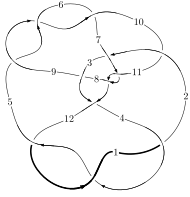
\includegraphics[width=112pt]{../../../GIT/diagram.site/Diagrams/png/1920_12a_1119.png}\\
\ \ \ A knot diagram\footnotemark}&
\allowdisplaybreaks
\textbf{Linearized knot diagam} \\
\cline{2-2}
 &
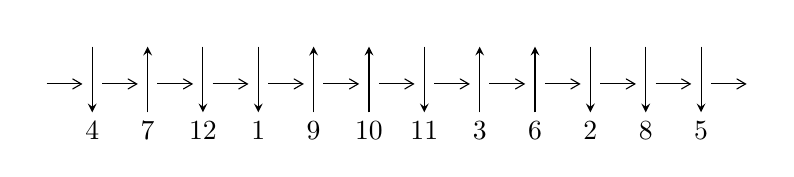
\begin{tikzpicture}[x=20pt, y=17pt]
	% nodes
	\node (C0) at (0, 0) {};
	\node (C1) at (1, 0) {};
	\node (C1U) at (1, +1) {};
	\node (C1D) at (1, -1) {4};

	\node (C2) at (2, 0) {};
	\node (C2U) at (2, +1) {};
	\node (C2D) at (2, -1) {7};

	\node (C3) at (3, 0) {};
	\node (C3U) at (3, +1) {};
	\node (C3D) at (3, -1) {12};

	\node (C4) at (4, 0) {};
	\node (C4U) at (4, +1) {};
	\node (C4D) at (4, -1) {1};

	\node (C5) at (5, 0) {};
	\node (C5U) at (5, +1) {};
	\node (C5D) at (5, -1) {9};

	\node (C6) at (6, 0) {};
	\node (C6U) at (6, +1) {};
	\node (C6D) at (6, -1) {10};

	\node (C7) at (7, 0) {};
	\node (C7U) at (7, +1) {};
	\node (C7D) at (7, -1) {11};

	\node (C8) at (8, 0) {};
	\node (C8U) at (8, +1) {};
	\node (C8D) at (8, -1) {3};

	\node (C9) at (9, 0) {};
	\node (C9U) at (9, +1) {};
	\node (C9D) at (9, -1) {6};

	\node (C10) at (10, 0) {};
	\node (C10U) at (10, +1) {};
	\node (C10D) at (10, -1) {2};

	\node (C11) at (11, 0) {};
	\node (C11U) at (11, +1) {};
	\node (C11D) at (11, -1) {8};

	\node (C12) at (12, 0) {};
	\node (C12U) at (12, +1) {};
	\node (C12D) at (12, -1) {5};
	\node (C13) at (13, 0) {};

	% arrows
	\draw[->,>={angle 60}]
	(C0) edge (C1) (C1) edge (C2) (C2) edge (C3) (C3) edge (C4) (C4) edge (C5) (C5) edge (C6) (C6) edge (C7) (C7) edge (C8) (C8) edge (C9) (C9) edge (C10) (C10) edge (C11) (C11) edge (C12) (C12) edge (C13) ;	\draw[->,>=stealth]
	(C1U) edge (C1D) (C2D) edge (C2U) (C3U) edge (C3D) (C4U) edge (C4D) (C5D) edge (C5U) (C6D) edge (C6U) (C7U) edge (C7D) (C8D) edge (C8U) (C9D) edge (C9U) (C10U) edge (C10D) (C11U) edge (C11D) (C12U) edge (C12D) ;
	\end{tikzpicture} \\
\hhline{~~} \\& 
\textbf{Solving Sequence} \\ \cline{2-2} 
 &
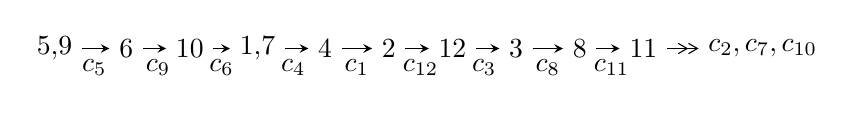
\begin{tikzpicture}[x=23pt, y=7pt]
	% node
	\node (A0) at (-1/8, 0) {5,9};
	\node (A1) at (1, 0) {6};
	\node (A2) at (2, 0) {10};
	\node (A3) at (49/16, 0) {1,7};
	\node (A4) at (33/8, 0) {4};
	\node (A5) at (41/8, 0) {2};
	\node (A6) at (49/8, 0) {12};
	\node (A7) at (57/8, 0) {3};
	\node (A8) at (65/8, 0) {8};
	\node (A9) at (73/8, 0) {11};
	\node (C1) at (1/2, -1) {$c_{5}$};
	\node (C2) at (3/2, -1) {$c_{9}$};
	\node (C3) at (5/2, -1) {$c_{6}$};
	\node (C4) at (29/8, -1) {$c_{4}$};
	\node (C5) at (37/8, -1) {$c_{1}$};
	\node (C6) at (45/8, -1) {$c_{12}$};
	\node (C7) at (53/8, -1) {$c_{3}$};
	\node (C8) at (61/8, -1) {$c_{8}$};
	\node (C9) at (69/8, -1) {$c_{11}$};
	\node (A10) at (11, 0) {$c_{2},c_{7},c_{10}$};

	% edge
	\draw[->,>=stealth]	
	(A0) edge (A1) (A1) edge (A2) (A2) edge (A3) (A3) edge (A4) (A4) edge (A5) (A5) edge (A6) (A6) edge (A7) (A7) edge (A8) (A8) edge (A9) ;
	\draw[->>,>={angle 60}]	
	(A9) edge (A10);
\end{tikzpicture} \\ 

\end{tabular} \\

\footnotetext{
The image of knot diagram is generated by the software ``\textbf{Draw programme}" developed by Andrew Bartholomew(\url{http://www.layer8.co.uk/maths/draw/index.htm\#Running-draw}), where we modified some parts for our purpose(\url{https://github.com/CATsTAILs/LinksPainter}).
}\phantom \\ \newline 
\centering \textbf{Ideals for irreducible components\footnotemark of $X_{\text{par}}$} 
 
\begin{align*}
I^u_{1}&=\langle 
-2.43683\times10^{139} u^{83}+3.15689\times10^{140} u^{82}+\cdots+5.45656\times10^{140} b-2.22182\times10^{139},\\
\phantom{I^u_{1}}&\phantom{= \langle  }2.34091\times10^{140} u^{83}-1.44662\times10^{141} u^{82}+\cdots+5.45656\times10^{140} a-5.49196\times10^{140},\;u^{84}-7 u^{83}+\cdots+7 u^2+1\rangle \\
\\
\end{align*}
\raggedright * 1 irreducible components of $\dim_{\mathbb{C}}=0$, with total 84 representations.\\
\footnotetext{All coefficients of polynomials are rational numbers. But the coefficients are sometimes approximated in decimal forms when there is not enough margin.}
\newpage
\renewcommand{\arraystretch}{1}
\centering \section*{I. $I^u_{1}= \langle -2.44\times10^{139} u^{83}+3.16\times10^{140} u^{82}+\cdots+5.46\times10^{140} b-2.22\times10^{139},\;2.34\times10^{140} u^{83}-1.45\times10^{141} u^{82}+\cdots+5.46\times10^{140} a-5.49\times10^{140},\;u^{84}-7 u^{83}+\cdots+7 u^2+1 \rangle$}
\flushleft \textbf{(i) Arc colorings}\\
\begin{tabular}{m{7pt} m{180pt} m{7pt} m{180pt} }
\flushright $a_{5}=$&$\begin{pmatrix}1\\0\end{pmatrix}$ \\
\flushright $a_{9}=$&$\begin{pmatrix}0\\u\end{pmatrix}$ \\
\flushright $a_{6}=$&$\begin{pmatrix}1\\- u^2\end{pmatrix}$ \\
\flushright $a_{10}=$&$\begin{pmatrix}u\\- u^3+u\end{pmatrix}$ \\
\flushright $a_{1}=$&$\begin{pmatrix}-0.429009 u^{83}+2.65116 u^{82}+\cdots+6.73479 u+1.00649\\0.0446588 u^{83}-0.578550 u^{82}+\cdots+0.0135038 u+0.0407184\end{pmatrix}$ \\
\flushright $a_{7}=$&$\begin{pmatrix}- u^2+1\\u^4-2 u^2\end{pmatrix}$ \\
\flushright $a_{4}=$&$\begin{pmatrix}0.334513 u^{83}-2.87235 u^{82}+\cdots+1.44740 u+2.70338\\-0.162239 u^{83}+0.872984 u^{82}+\cdots+1.58318 u-0.361124\end{pmatrix}$ \\
\flushright $a_{2}=$&$\begin{pmatrix}-0.133440 u^{83}-0.707253 u^{82}+\cdots+11.9226 u+0.535960\\-0.167963 u^{83}+1.28402 u^{82}+\cdots+1.04242 u-1.33717\end{pmatrix}$ \\
\flushright $a_{12}=$&$\begin{pmatrix}-0.384350 u^{83}+2.07261 u^{82}+\cdots+6.74830 u+1.04721\\0.0446588 u^{83}-0.578550 u^{82}+\cdots+0.0135038 u+0.0407184\end{pmatrix}$ \\
\flushright $a_{3}=$&$\begin{pmatrix}-0.288339 u^{83}+0.698691 u^{82}+\cdots+11.0956 u+0.146923\\-0.197313 u^{83}+1.54442 u^{82}+\cdots+0.418755 u-1.18254\end{pmatrix}$ \\
\flushright $a_{8}=$&$\begin{pmatrix}0.911994 u^{83}-5.64628 u^{82}+\cdots-10.3785 u-5.24643\\0.158497 u^{83}-0.788027 u^{82}+\cdots+2.54815 u+0.342618\end{pmatrix}$ \\
\flushright $a_{11}=$&$\begin{pmatrix}1.62663 u^{83}-11.7707 u^{82}+\cdots-6.84432 u-3.89169\\0.694473 u^{83}-4.03384 u^{82}+\cdots+1.64447 u-0.0378106\end{pmatrix}$\\&\end{tabular}
\flushleft \textbf{(ii) Obstruction class $= -1$}\\~\\
\flushleft \textbf{(iii) Cusp Shapes $= -6.53695 u^{83}+39.5178 u^{82}+\cdots+24.3239 u-1.59872$}\\~\\
\newpage\renewcommand{\arraystretch}{1}
\flushleft \textbf{(iv) u-Polynomials at the component}\newline \\
\begin{tabular}{m{50pt}|m{274pt}}
Crossings & \hspace{64pt}u-Polynomials at each crossing \\
\hline $$\begin{aligned}c_{1},c_{4},c_{12}\end{aligned}$$&$\begin{aligned}
&u^{84}- u^{83}+\cdots-14 u+1
\end{aligned}$\\
\hline $$\begin{aligned}c_{2}\end{aligned}$$&$\begin{aligned}
&u^{84}+3 u^{83}+\cdots+4 u+1
\end{aligned}$\\
\hline $$\begin{aligned}c_{3}\end{aligned}$$&$\begin{aligned}
&u^{84}+u^{83}+\cdots-43278 u+4801
\end{aligned}$\\
\hline $$\begin{aligned}c_{5},c_{6},c_{9}\end{aligned}$$&$\begin{aligned}
&u^{84}-7 u^{83}+\cdots+7 u^2+1
\end{aligned}$\\
\hline $$\begin{aligned}c_{7},c_{11}\end{aligned}$$&$\begin{aligned}
&u^{84}+u^{83}+\cdots+7 u^2+1
\end{aligned}$\\
\hline $$\begin{aligned}c_{8}\end{aligned}$$&$\begin{aligned}
&u^{84}- u^{83}+\cdots-6188 u+3431
\end{aligned}$\\
\hline $$\begin{aligned}c_{10}\end{aligned}$$&$\begin{aligned}
&u^{84}+5 u^{83}+\cdots-46 u+13
\end{aligned}$\\
\hline
\end{tabular}\\~\\
\newpage\renewcommand{\arraystretch}{1}
\flushleft \textbf{(v) Riley Polynomials at the component}\newline \\
\begin{tabular}{m{50pt}|m{274pt}}
Crossings & \hspace{64pt}Riley Polynomials at each crossing \\
\hline $$\begin{aligned}c_{1},c_{4},c_{12}\end{aligned}$$&$\begin{aligned}
&y^{84}+73 y^{83}+\cdots-102 y+1
\end{aligned}$\\
\hline $$\begin{aligned}c_{2}\end{aligned}$$&$\begin{aligned}
&y^{84}-7 y^{83}+\cdots-78 y+1
\end{aligned}$\\
\hline $$\begin{aligned}c_{3}\end{aligned}$$&$\begin{aligned}
&y^{84}-19 y^{83}+\cdots-2061501350 y+23049601
\end{aligned}$\\
\hline $$\begin{aligned}c_{5},c_{6},c_{9}\end{aligned}$$&$\begin{aligned}
&y^{84}-83 y^{83}+\cdots+14 y+1
\end{aligned}$\\
\hline $$\begin{aligned}c_{7},c_{11}\end{aligned}$$&$\begin{aligned}
&y^{84}-59 y^{83}+\cdots+14 y+1
\end{aligned}$\\
\hline $$\begin{aligned}c_{8}\end{aligned}$$&$\begin{aligned}
&y^{84}-211 y^{83}+\cdots+403051910 y+11771761
\end{aligned}$\\
\hline $$\begin{aligned}c_{10}\end{aligned}$$&$\begin{aligned}
&y^{84}-259 y^{83}+\cdots+32802 y+169
\end{aligned}$\\
\hline
\end{tabular}\\~\\
\newpage\flushleft \textbf{(vi) Complex Volumes and Cusp Shapes}
$$\begin{array}{c|c|c}  
\text{Solutions to }I^u_{1}& \I (\text{vol} + \sqrt{-1}CS) & \text{Cusp shape}\\
 \hline 
\begin{aligned}
u &= -0.558103 + 0.837786 I \\
a &= \phantom{-}1.52550 - 1.04449 I \\
b &= \phantom{-}0.32653 + 1.38845 I\end{aligned}
 & -0.28320 - 12.83660 I & \phantom{-0.000000 } 0 \\ \hline\begin{aligned}
u &= -0.558103 - 0.837786 I \\
a &= \phantom{-}1.52550 + 1.04449 I \\
b &= \phantom{-}0.32653 - 1.38845 I\end{aligned}
 & -0.28320 + 12.83660 I & \phantom{-0.000000 } 0 \\ \hline\begin{aligned}
u &= -0.639681 + 0.783616 I \\
a &= \phantom{-}0.411406 - 0.299400 I \\
b &= \phantom{-}0.711341 - 0.142714 I\end{aligned}
 & -4.95491 + 3.53314 I & \phantom{-0.000000 } 0 \\ \hline\begin{aligned}
u &= -0.639681 - 0.783616 I \\
a &= \phantom{-}0.411406 + 0.299400 I \\
b &= \phantom{-}0.711341 + 0.142714 I\end{aligned}
 & -4.95491 - 3.53314 I & \phantom{-0.000000 } 0 \\ \hline\begin{aligned}
u &= -0.747659 + 0.597758 I \\
a &= \phantom{-}1.51169 - 1.14560 I \\
b &= \phantom{-}0.227897 + 1.113580 I\end{aligned}
 & -2.10479 + 0.01557 I & \phantom{-0.000000 } 0 \\ \hline\begin{aligned}
u &= -0.747659 - 0.597758 I \\
a &= \phantom{-}1.51169 + 1.14560 I \\
b &= \phantom{-}0.227897 - 1.113580 I\end{aligned}
 & -2.10479 - 0.01557 I & \phantom{-0.000000 } 0 \\ \hline\begin{aligned}
u &= -0.490660 + 0.800323 I \\
a &= \phantom{-}0.681388 - 0.567665 I \\
b &= \phantom{-}0.792584 + 0.213001 I\end{aligned}
 & -5.35864 - 8.79455 I & \phantom{-0.000000 } 0 \\ \hline\begin{aligned}
u &= -0.490660 - 0.800323 I \\
a &= \phantom{-}0.681388 + 0.567665 I \\
b &= \phantom{-}0.792584 - 0.213001 I\end{aligned}
 & -5.35864 + 8.79455 I & \phantom{-0.000000 } 0 \\ \hline\begin{aligned}
u &= \phantom{-}0.401609 + 0.848172 I \\
a &= \phantom{-}0.805169 + 0.380180 I \\
b &= \phantom{-}0.613779 - 0.176501 I\end{aligned}
 & -0.43669 + 3.36220 I & \phantom{-0.000000 } 0 \\ \hline\begin{aligned}
u &= \phantom{-}0.401609 - 0.848172 I \\
a &= \phantom{-}0.805169 - 0.380180 I \\
b &= \phantom{-}0.613779 + 0.176501 I\end{aligned}
 & -0.43669 - 3.36220 I & \phantom{-0.000000 } 0\\
 \hline 
 \end{array}$$\newpage$$\begin{array}{c|c|c}  
\text{Solutions to }I^u_{1}& \I (\text{vol} + \sqrt{-1}CS) & \text{Cusp shape}\\
 \hline 
\begin{aligned}
u &= -0.593656 + 0.901541 I \\
a &= \phantom{-}0.177974 + 0.754728 I \\
b &= \phantom{-}0.288082 - 1.348880 I\end{aligned}
 & -0.24649 + 7.15365 I & \phantom{-0.000000 } 0 \\ \hline\begin{aligned}
u &= -0.593656 - 0.901541 I \\
a &= \phantom{-}0.177974 - 0.754728 I \\
b &= \phantom{-}0.288082 + 1.348880 I\end{aligned}
 & -0.24649 - 7.15365 I & \phantom{-0.000000 } 0 \\ \hline\begin{aligned}
u &= \phantom{-}1.088040 + 0.044118 I \\
a &= \phantom{-}1.15502 + 1.02120 I \\
b &= -0.028874 - 1.253000 I\end{aligned}
 & \phantom{-}5.55571 + 0.01357 I & \phantom{-0.000000 } 0 \\ \hline\begin{aligned}
u &= \phantom{-}1.088040 - 0.044118 I \\
a &= \phantom{-}1.15502 - 1.02120 I \\
b &= -0.028874 + 1.253000 I\end{aligned}
 & \phantom{-}5.55571 - 0.01357 I & \phantom{-0.000000 } 0 \\ \hline\begin{aligned}
u &= \phantom{-}0.523355 + 0.968000 I \\
a &= \phantom{-}1.40292 + 0.93077 I \\
b &= \phantom{-}0.248772 - 1.359780 I\end{aligned}
 & \phantom{-}4.42501 + 6.53157 I & \phantom{-0.000000 } 0 \\ \hline\begin{aligned}
u &= \phantom{-}0.523355 - 0.968000 I \\
a &= \phantom{-}1.40292 - 0.93077 I \\
b &= \phantom{-}0.248772 + 1.359780 I\end{aligned}
 & \phantom{-}4.42501 - 6.53157 I & \phantom{-0.000000 } 0 \\ \hline\begin{aligned}
u &= \phantom{-}0.985199 + 0.608775 I \\
a &= \phantom{-}0.194220 - 1.206160 I \\
b &= \phantom{-}0.134578 + 1.326750 I\end{aligned}
 & \phantom{-}5.97791 - 0.32219 I & \phantom{-0.000000 } 0 \\ \hline\begin{aligned}
u &= \phantom{-}0.985199 - 0.608775 I \\
a &= \phantom{-}0.194220 + 1.206160 I \\
b &= \phantom{-}0.134578 - 1.326750 I\end{aligned}
 & \phantom{-}5.97791 + 0.32219 I & \phantom{-0.000000 } 0 \\ \hline\begin{aligned}
u &= -0.014818 + 0.841024 I \\
a &= \phantom{-}1.022770 - 0.141577 I \\
b &= \phantom{-}0.101645 + 1.273120 I\end{aligned}
 & \phantom{-}2.45064 + 1.09496 I & \phantom{-0.000000 } 0. - 4.87467 I \\ \hline\begin{aligned}
u &= -0.014818 - 0.841024 I \\
a &= \phantom{-}1.022770 + 0.141577 I \\
b &= \phantom{-}0.101645 - 1.273120 I\end{aligned}
 & \phantom{-}2.45064 - 1.09496 I & \phantom{-0.000000 -}0. + 4.87467 I\\
 \hline 
 \end{array}$$\newpage$$\begin{array}{c|c|c}  
\text{Solutions to }I^u_{1}& \I (\text{vol} + \sqrt{-1}CS) & \text{Cusp shape}\\
 \hline 
\begin{aligned}
u &= -0.403808 + 0.710608 I \\
a &= \phantom{-}0.183228 + 0.122343 I \\
b &= \phantom{-}0.390587 - 0.945271 I\end{aligned}
 & -3.07733 - 4.49445 I & \phantom{-0.000000 -}0. + 4.03751 I \\ \hline\begin{aligned}
u &= -0.403808 - 0.710608 I \\
a &= \phantom{-}0.183228 - 0.122343 I \\
b &= \phantom{-}0.390587 + 0.945271 I\end{aligned}
 & -3.07733 + 4.49445 I & \phantom{-0.000000 } 0. - 4.03751 I \\ \hline\begin{aligned}
u &= -0.609196 + 0.406672 I \\
a &= -0.28476 + 1.62479 I \\
b &= -0.04981 - 1.43688 I\end{aligned}
 & \phantom{-}4.61918 - 4.68420 I & \phantom{-}2.69222 + 7.52303 I \\ \hline\begin{aligned}
u &= -0.609196 - 0.406672 I \\
a &= -0.28476 - 1.62479 I \\
b &= -0.04981 + 1.43688 I\end{aligned}
 & \phantom{-}4.61918 + 4.68420 I & \phantom{-}2.69222 - 7.52303 I \\ \hline\begin{aligned}
u &= \phantom{-}1.31401\phantom{ +0.000000I} \\
a &= \phantom{-}0.437229\phantom{ +0.000000I} \\
b &= -1.04347\phantom{ +0.000000I}\end{aligned}
 & -1.24406\phantom{ +0.000000I} & \phantom{-0.000000 } 0 \\ \hline\begin{aligned}
u &= -1.330080 + 0.068788 I \\
a &= \phantom{-}0.429993 + 0.933227 I \\
b &= -0.903437 - 0.502221 I\end{aligned}
 & -0.39209 - 2.89833 I & \phantom{-0.000000 } 0 \\ \hline\begin{aligned}
u &= -1.330080 - 0.068788 I \\
a &= \phantom{-}0.429993 - 0.933227 I \\
b &= -0.903437 + 0.502221 I\end{aligned}
 & -0.39209 + 2.89833 I & \phantom{-0.000000 } 0 \\ \hline\begin{aligned}
u &= -1.346290 + 0.084631 I \\
a &= -0.465672 + 0.572476 I \\
b &= -0.270534 - 1.164230 I\end{aligned}
 & \phantom{-}6.20610 - 3.71389 I & \phantom{-0.000000 } 0 \\ \hline\begin{aligned}
u &= -1.346290 - 0.084631 I \\
a &= -0.465672 - 0.572476 I \\
b &= -0.270534 + 1.164230 I\end{aligned}
 & \phantom{-}6.20610 + 3.71389 I & \phantom{-0.000000 } 0 \\ \hline\begin{aligned}
u &= \phantom{-}0.470607 + 0.437247 I \\
a &= \phantom{-}0.379162 - 0.111252 I \\
b &= \phantom{-}0.167310 + 0.380669 I\end{aligned}
 & \phantom{-}1.018620 + 0.865781 I & \phantom{-}4.46908 - 2.51048 I\\
 \hline 
 \end{array}$$\newpage$$\begin{array}{c|c|c}  
\text{Solutions to }I^u_{1}& \I (\text{vol} + \sqrt{-1}CS) & \text{Cusp shape}\\
 \hline 
\begin{aligned}
u &= \phantom{-}0.470607 - 0.437247 I \\
a &= \phantom{-}0.379162 + 0.111252 I \\
b &= \phantom{-}0.167310 - 0.380669 I\end{aligned}
 & \phantom{-}1.018620 - 0.865781 I & \phantom{-}4.46908 + 2.51048 I \\ \hline\begin{aligned}
u &= \phantom{-}1.357310 + 0.113910 I \\
a &= -0.08709 - 1.41361 I \\
b &= -0.595285 + 1.116090 I\end{aligned}
 & \phantom{-}2.14730 + 5.65478 I & \phantom{-0.000000 } 0 \\ \hline\begin{aligned}
u &= \phantom{-}1.357310 - 0.113910 I \\
a &= -0.08709 + 1.41361 I \\
b &= -0.595285 - 1.116090 I\end{aligned}
 & \phantom{-}2.14730 - 5.65478 I & \phantom{-0.000000 } 0 \\ \hline\begin{aligned}
u &= -1.36225\phantom{ +0.000000I} \\
a &= -0.619840\phantom{ +0.000000I} \\
b &= -0.737594\phantom{ +0.000000I}\end{aligned}
 & \phantom{-}2.64928\phantom{ +0.000000I} & \phantom{-0.000000 } 0 \\ \hline\begin{aligned}
u &= \phantom{-}1.372000 + 0.056138 I \\
a &= \phantom{-}0.166578 - 1.098660 I \\
b &= -0.589738 + 0.319680 I\end{aligned}
 & \phantom{-}3.44980 + 1.64919 I & \phantom{-0.000000 } 0 \\ \hline\begin{aligned}
u &= \phantom{-}1.372000 - 0.056138 I \\
a &= \phantom{-}0.166578 + 1.098660 I \\
b &= -0.589738 - 0.319680 I\end{aligned}
 & \phantom{-}3.44980 - 1.64919 I & \phantom{-0.000000 } 0 \\ \hline\begin{aligned}
u &= -1.40478\phantom{ +0.000000I} \\
a &= -9.12724\phantom{ +0.000000I} \\
b &= -0.576785\phantom{ +0.000000I}\end{aligned}
 & \phantom{-}2.15827\phantom{ +0.000000I} & \phantom{-0.000000 } 0 \\ \hline\begin{aligned}
u &= -1.414000 + 0.020024 I \\
a &= -10.33470 + 3.36484 I \\
b &= -0.218790 - 1.310170 I\end{aligned}
 & \phantom{-}6.31232 - 2.86771 I & \phantom{-0.000000 } 0 \\ \hline\begin{aligned}
u &= -1.414000 - 0.020024 I \\
a &= -10.33470 - 3.36484 I \\
b &= -0.218790 + 1.310170 I\end{aligned}
 & \phantom{-}6.31232 + 2.86771 I & \phantom{-0.000000 } 0 \\ \hline\begin{aligned}
u &= -1.41705 + 0.12490 I \\
a &= -0.72952 + 2.35259 I \\
b &= -0.36926 - 1.49647 I\end{aligned}
 & \phantom{-}5.91677 - 7.57306 I & \phantom{-0.000000 } 0\\
 \hline 
 \end{array}$$\newpage$$\begin{array}{c|c|c}  
\text{Solutions to }I^u_{1}& \I (\text{vol} + \sqrt{-1}CS) & \text{Cusp shape}\\
 \hline 
\begin{aligned}
u &= -1.41705 - 0.12490 I \\
a &= -0.72952 - 2.35259 I \\
b &= -0.36926 + 1.49647 I\end{aligned}
 & \phantom{-}5.91677 + 7.57306 I & \phantom{-0.000000 } 0 \\ \hline\begin{aligned}
u &= \phantom{-}1.43896 + 0.09315 I \\
a &= -1.15853 - 2.79825 I \\
b &= -0.24915 + 1.42600 I\end{aligned}
 & \phantom{-}9.04553 + 4.79524 I & \phantom{-0.000000 } 0 \\ \hline\begin{aligned}
u &= \phantom{-}1.43896 - 0.09315 I \\
a &= -1.15853 + 2.79825 I \\
b &= -0.24915 - 1.42600 I\end{aligned}
 & \phantom{-}9.04553 - 4.79524 I & \phantom{-0.000000 } 0 \\ \hline\begin{aligned}
u &= \phantom{-}1.42046 + 0.37578 I \\
a &= \phantom{-}0.456228 + 0.488501 I \\
b &= \phantom{-}0.548985 - 0.149764 I\end{aligned}
 & \phantom{-}2.49026 + 1.60685 I & \phantom{-0.000000 } 0 \\ \hline\begin{aligned}
u &= \phantom{-}1.42046 - 0.37578 I \\
a &= \phantom{-}0.456228 - 0.488501 I \\
b &= \phantom{-}0.548985 + 0.149764 I\end{aligned}
 & \phantom{-}2.49026 - 1.60685 I & \phantom{-0.000000 } 0 \\ \hline\begin{aligned}
u &= -0.204867 + 0.486225 I \\
a &= -0.343437 + 0.220412 I \\
b &= -0.482066 - 0.851406 I\end{aligned}
 & -2.67638 - 3.53656 I & -7.87807 + 8.61174 I \\ \hline\begin{aligned}
u &= -0.204867 - 0.486225 I \\
a &= -0.343437 - 0.220412 I \\
b &= -0.482066 + 0.851406 I\end{aligned}
 & -2.67638 + 3.53656 I & -7.87807 - 8.61174 I \\ \hline\begin{aligned}
u &= \phantom{-}1.47597\phantom{ +0.000000I} \\
a &= \phantom{-}0.594054\phantom{ +0.000000I} \\
b &= \phantom{-}0.100712\phantom{ +0.000000I}\end{aligned}
 & \phantom{-}3.39757\phantom{ +0.000000I} & \phantom{-0.000000 } 0 \\ \hline\begin{aligned}
u &= \phantom{-}0.287913 + 0.434694 I \\
a &= -1.36655 - 0.68485 I \\
b &= -0.35900 + 1.38494 I\end{aligned}
 & \phantom{-}0.44827 + 5.59393 I & -4.07425 - 9.66974 I \\ \hline\begin{aligned}
u &= \phantom{-}0.287913 - 0.434694 I \\
a &= -1.36655 + 0.68485 I \\
b &= -0.35900 - 1.38494 I\end{aligned}
 & \phantom{-}0.44827 - 5.59393 I & -4.07425 + 9.66974 I\\
 \hline 
 \end{array}$$\newpage$$\begin{array}{c|c|c}  
\text{Solutions to }I^u_{1}& \I (\text{vol} + \sqrt{-1}CS) & \text{Cusp shape}\\
 \hline 
\begin{aligned}
u &= -1.47315 + 0.20651 I \\
a &= -0.143376 + 0.617668 I \\
b &= \phantom{-}0.401164 - 0.693355 I\end{aligned}
 & \phantom{-}7.23640 - 3.44789 I & \phantom{-0.000000 } 0 \\ \hline\begin{aligned}
u &= -1.47315 - 0.20651 I \\
a &= -0.143376 - 0.617668 I \\
b &= \phantom{-}0.401164 + 0.693355 I\end{aligned}
 & \phantom{-}7.23640 + 3.44789 I & \phantom{-0.000000 } 0 \\ \hline\begin{aligned}
u &= \phantom{-}1.47977 + 0.24770 I \\
a &= -0.358315 - 0.779942 I \\
b &= \phantom{-}0.534813 + 0.884353 I\end{aligned}
 & \phantom{-}3.04368 + 7.95765 I & \phantom{-0.000000 } 0 \\ \hline\begin{aligned}
u &= \phantom{-}1.47977 - 0.24770 I \\
a &= -0.358315 + 0.779942 I \\
b &= \phantom{-}0.534813 - 0.884353 I\end{aligned}
 & \phantom{-}3.04368 - 7.95765 I & \phantom{-0.000000 } 0 \\ \hline\begin{aligned}
u &= -0.344988 + 0.334848 I \\
a &= \phantom{-}1.92138 + 0.14934 I \\
b &= -0.197517 + 0.346890 I\end{aligned}
 & -1.92460 + 0.99564 I & -1.96608 + 2.11328 I \\ \hline\begin{aligned}
u &= -0.344988 - 0.334848 I \\
a &= \phantom{-}1.92138 - 0.14934 I \\
b &= -0.197517 - 0.346890 I\end{aligned}
 & -1.92460 - 0.99564 I & -1.96608 - 2.11328 I \\ \hline\begin{aligned}
u &= \phantom{-}1.51666 + 0.14625 I \\
a &= -0.29716 - 2.66877 I \\
b &= -0.00970 + 1.54752 I\end{aligned}
 & \phantom{-}11.56010 + 6.78696 I & \phantom{-0.000000 } 0 \\ \hline\begin{aligned}
u &= \phantom{-}1.51666 - 0.14625 I \\
a &= -0.29716 + 2.66877 I \\
b &= -0.00970 - 1.54752 I\end{aligned}
 & \phantom{-}11.56010 - 6.78696 I & \phantom{-0.000000 } 0 \\ \hline\begin{aligned}
u &= -1.49761 + 0.29399 I \\
a &= \phantom{-}0.233342 - 0.820168 I \\
b &= \phantom{-}0.726980 + 0.278450 I\end{aligned}
 & \phantom{-}5.75269 - 7.44281 I & \phantom{-0.000000 } 0 \\ \hline\begin{aligned}
u &= -1.49761 - 0.29399 I \\
a &= \phantom{-}0.233342 + 0.820168 I \\
b &= \phantom{-}0.726980 - 0.278450 I\end{aligned}
 & \phantom{-}5.75269 + 7.44281 I & \phantom{-0.000000 } 0\\
 \hline 
 \end{array}$$\newpage$$\begin{array}{c|c|c}  
\text{Solutions to }I^u_{1}& \I (\text{vol} + \sqrt{-1}CS) & \text{Cusp shape}\\
 \hline 
\begin{aligned}
u &= \phantom{-}1.51599 + 0.28498 I \\
a &= \phantom{-}0.058636 + 0.886807 I \\
b &= \phantom{-}0.835240 - 0.276491 I\end{aligned}
 & \phantom{-}1.14844 + 12.74900 I & \phantom{-0.000000 } 0 \\ \hline\begin{aligned}
u &= \phantom{-}1.51599 - 0.28498 I \\
a &= \phantom{-}0.058636 - 0.886807 I \\
b &= \phantom{-}0.835240 + 0.276491 I\end{aligned}
 & \phantom{-}1.14844 - 12.74900 I & \phantom{-0.000000 } 0 \\ \hline\begin{aligned}
u &= -0.012086 + 0.442740 I \\
a &= \phantom{-}0.89158 + 2.28803 I \\
b &= -0.162190 + 1.277820 I\end{aligned}
 & \phantom{-}2.28626 + 2.04027 I & -3.92912 - 5.24188 I \\ \hline\begin{aligned}
u &= -0.012086 - 0.442740 I \\
a &= \phantom{-}0.89158 - 2.28803 I \\
b &= -0.162190 - 1.277820 I\end{aligned}
 & \phantom{-}2.28626 - 2.04027 I & -3.92912 + 5.24188 I \\ \hline\begin{aligned}
u &= \phantom{-}0.076173 + 0.427342 I \\
a &= -0.694821 - 0.381532 I \\
b &= -0.857353 + 0.238672 I\end{aligned}
 & -4.65098 + 1.20835 I & -15.0329 - 4.8481 I \\ \hline\begin{aligned}
u &= \phantom{-}0.076173 - 0.427342 I \\
a &= -0.694821 + 0.381532 I \\
b &= -0.857353 - 0.238672 I\end{aligned}
 & -4.65098 - 1.20835 I & -15.0329 + 4.8481 I \\ \hline\begin{aligned}
u &= -1.56700 + 0.14380 I \\
a &= -0.02967 + 2.52214 I \\
b &= \phantom{-}0.07633 - 1.46544 I\end{aligned}
 & \phantom{-}14.1292 - 2.0376 I & \phantom{-0.000000 } 0 \\ \hline\begin{aligned}
u &= -1.56700 - 0.14380 I \\
a &= -0.02967 - 2.52214 I \\
b &= \phantom{-}0.07633 + 1.46544 I\end{aligned}
 & \phantom{-}14.1292 + 2.0376 I & \phantom{-0.000000 } 0 \\ \hline\begin{aligned}
u &= \phantom{-}1.54885 + 0.29519 I \\
a &= \phantom{-}1.34400 + 2.12210 I \\
b &= \phantom{-}0.33964 - 1.42580 I\end{aligned}
 & \phantom{-}6.5668 + 16.9923 I & \phantom{-0.000000 } 0 \\ \hline\begin{aligned}
u &= \phantom{-}1.54885 - 0.29519 I \\
a &= \phantom{-}1.34400 - 2.12210 I \\
b &= \phantom{-}0.33964 + 1.42580 I\end{aligned}
 & \phantom{-}6.5668 - 16.9923 I & \phantom{-0.000000 } 0\\
 \hline 
 \end{array}$$\newpage$$\begin{array}{c|c|c}  
\text{Solutions to }I^u_{1}& \I (\text{vol} + \sqrt{-1}CS) & \text{Cusp shape}\\
 \hline 
\begin{aligned}
u &= -1.54618 + 0.32454 I \\
a &= \phantom{-}1.38269 - 2.01148 I \\
b &= \phantom{-}0.29004 + 1.41078 I\end{aligned}
 & \phantom{-}11.1318 - 11.1393 I & \phantom{-0.000000 } 0 \\ \hline\begin{aligned}
u &= -1.54618 - 0.32454 I \\
a &= \phantom{-}1.38269 + 2.01148 I \\
b &= \phantom{-}0.29004 - 1.41078 I\end{aligned}
 & \phantom{-}11.1318 + 11.1393 I & \phantom{-0.000000 } 0 \\ \hline\begin{aligned}
u &= \phantom{-}0.345350 + 0.231832 I \\
a &= \phantom{-}4.98640 + 1.68201 I \\
b &= -0.262208 - 1.299920 I\end{aligned}
 & \phantom{-}0.91964 - 3.32129 I & \phantom{-}6.11652 - 8.60509 I \\ \hline\begin{aligned}
u &= \phantom{-}0.345350 - 0.231832 I \\
a &= \phantom{-}4.98640 - 1.68201 I \\
b &= -0.262208 + 1.299920 I\end{aligned}
 & \phantom{-}0.91964 + 3.32129 I & \phantom{-}6.11652 + 8.60509 I \\ \hline\begin{aligned}
u &= -0.300231 + 0.276423 I \\
a &= -2.82551 + 2.03371 I \\
b &= -0.229473 - 1.345730 I\end{aligned}
 & \phantom{-}3.36187 - 3.41278 I & -0.247336 + 1.025326 I \\ \hline\begin{aligned}
u &= -0.300231 - 0.276423 I \\
a &= -2.82551 - 2.03371 I \\
b &= -0.229473 + 1.345730 I\end{aligned}
 & \phantom{-}3.36187 + 3.41278 I & -0.247336 - 1.025326 I \\ \hline\begin{aligned}
u &= \phantom{-}1.61987\phantom{ +0.000000I} \\
a &= \phantom{-}0.207346\phantom{ +0.000000I} \\
b &= \phantom{-}0.397949\phantom{ +0.000000I}\end{aligned}
 & \phantom{-}3.31098\phantom{ +0.000000I} & \phantom{-0.000000 } 0 \\ \hline\begin{aligned}
u &= \phantom{-}1.56407 + 0.45989 I \\
a &= \phantom{-}1.32437 + 1.73919 I \\
b &= \phantom{-}0.223403 - 1.352190 I\end{aligned}
 & \phantom{-}7.25184 + 4.47084 I & \phantom{-0.000000 } 0 \\ \hline\begin{aligned}
u &= \phantom{-}1.56407 - 0.45989 I \\
a &= \phantom{-}1.32437 - 1.73919 I \\
b &= \phantom{-}0.223403 + 1.352190 I\end{aligned}
 & \phantom{-}7.25184 - 4.47084 I & \phantom{-0.000000 } 0 \\ \hline\begin{aligned}
u &= \phantom{-}0.316396\phantom{ +0.000000I} \\
a &= \phantom{-}4.76803\phantom{ +0.000000I} \\
b &= -0.657423\phantom{ +0.000000I}\end{aligned}
 & -3.17231\phantom{ +0.000000I} & \phantom{-}16.2440\phantom{ +0.000000I}\\
 \hline 
 \end{array}$$\newpage$$\begin{array}{c|c|c}  
\text{Solutions to }I^u_{1}& \I (\text{vol} + \sqrt{-1}CS) & \text{Cusp shape}\\
 \hline 
\begin{aligned}
u &= -0.116009 + 0.290071 I \\
a &= -1.05692 + 1.73060 I \\
b &= -0.574135 - 0.102366 I\end{aligned}
 & -1.248270 - 0.474713 I & -7.55961 + 0.17216 I \\ \hline\begin{aligned}
u &= -0.116009 - 0.290071 I \\
a &= -1.05692 - 1.73060 I \\
b &= -0.574135 + 0.102366 I\end{aligned}
 & -1.248270 + 0.474713 I & -7.55961 - 0.17216 I \\ \hline\begin{aligned}
u &= \phantom{-}1.75518 + 0.17068 I \\
a &= \phantom{-}0.40063 - 1.98817 I \\
b &= \phantom{-}0.187126 + 1.339880 I\end{aligned}
 & \phantom{-}7.78775 - 2.29126 I & \phantom{-0.000000 } 0 \\ \hline\begin{aligned}
u &= \phantom{-}1.75518 - 0.17068 I \\
a &= \phantom{-}0.40063 + 1.98817 I \\
b &= \phantom{-}0.187126 - 1.339880 I\end{aligned}
 & \phantom{-}7.78775 + 2.29126 I & \phantom{-0.000000 } 0\\
 \hline 
 \end{array}$$\newpage
\newpage\renewcommand{\arraystretch}{1}
\centering \section*{ II. u-Polynomials}
\begin{tabular}{m{50pt}|m{274pt}}
Crossings & \hspace{64pt}u-Polynomials at each crossing \\
\hline $$\begin{aligned}c_{1},c_{4},c_{12}\end{aligned}$$&$\begin{aligned}
&u^{84}- u^{83}+\cdots-14 u+1
\end{aligned}$\\
\hline $$\begin{aligned}c_{2}\end{aligned}$$&$\begin{aligned}
&u^{84}+3 u^{83}+\cdots+4 u+1
\end{aligned}$\\
\hline $$\begin{aligned}c_{3}\end{aligned}$$&$\begin{aligned}
&u^{84}+u^{83}+\cdots-43278 u+4801
\end{aligned}$\\
\hline $$\begin{aligned}c_{5},c_{6},c_{9}\end{aligned}$$&$\begin{aligned}
&u^{84}-7 u^{83}+\cdots+7 u^2+1
\end{aligned}$\\
\hline $$\begin{aligned}c_{7},c_{11}\end{aligned}$$&$\begin{aligned}
&u^{84}+u^{83}+\cdots+7 u^2+1
\end{aligned}$\\
\hline $$\begin{aligned}c_{8}\end{aligned}$$&$\begin{aligned}
&u^{84}- u^{83}+\cdots-6188 u+3431
\end{aligned}$\\
\hline $$\begin{aligned}c_{10}\end{aligned}$$&$\begin{aligned}
&u^{84}+5 u^{83}+\cdots-46 u+13
\end{aligned}$\\
\hline
\end{tabular}\newpage\renewcommand{\arraystretch}{1}
\centering \section*{ III. Riley Polynomials}
\begin{tabular}{m{50pt}|m{274pt}}
Crossings & \hspace{64pt}Riley Polynomials at each crossing \\
\hline $$\begin{aligned}c_{1},c_{4},c_{12}\end{aligned}$$&$\begin{aligned}
&y^{84}+73 y^{83}+\cdots-102 y+1
\end{aligned}$\\
\hline $$\begin{aligned}c_{2}\end{aligned}$$&$\begin{aligned}
&y^{84}-7 y^{83}+\cdots-78 y+1
\end{aligned}$\\
\hline $$\begin{aligned}c_{3}\end{aligned}$$&$\begin{aligned}
&y^{84}-19 y^{83}+\cdots-2061501350 y+23049601
\end{aligned}$\\
\hline $$\begin{aligned}c_{5},c_{6},c_{9}\end{aligned}$$&$\begin{aligned}
&y^{84}-83 y^{83}+\cdots+14 y+1
\end{aligned}$\\
\hline $$\begin{aligned}c_{7},c_{11}\end{aligned}$$&$\begin{aligned}
&y^{84}-59 y^{83}+\cdots+14 y+1
\end{aligned}$\\
\hline $$\begin{aligned}c_{8}\end{aligned}$$&$\begin{aligned}
&y^{84}-211 y^{83}+\cdots+403051910 y+11771761
\end{aligned}$\\
\hline $$\begin{aligned}c_{10}\end{aligned}$$&$\begin{aligned}
&y^{84}-259 y^{83}+\cdots+32802 y+169
\end{aligned}$\\
\hline
\end{tabular}
\vskip 2pc
\end{document}